\cotefile{151}
\scanpage{32}
de \uline{locale trivialité normale} a un rôle
à jouer (celle de lissité \unsure{restant} comme
devant techniquement inutile \deleted{\unsure{?}}, son rôle
étant plutôt de nature heuristique ...).

\deleted{\unsure{On}} On doit se débrouiller, dans ce cas,
pour démontrer que les propriétés homo-
topiques de l'inclusion $V^*_{Y,X}\subset V_{Y,X}$
\margin{\diagram{\begin{tikzcd}[row sep=small]
{} \arrow[d, shift left=.4ex, "{\unsure{\text{homo-topisme}}}"'] \\
Y \arrow[u, shift left=.4ex]
\end{tikzcd}}\deleted{\unsure{Id}}}
sont celles d'une \uline{fibration}
\uline{localement triviale de fibre} $V^*_{z,\unsure{Z|X}}$ :

\noindent (11) $V^*_{Y,X}\longrightarrow V_{Y,X}$ est une ``fibration
homotopique'' de fibre $V^*_{z,X}$,
de base $Y\xrightarrow{\approx\,\mathrm{homot.}} V_{Y,X}$

--- et c'est cela qui devrait même,
dans le contexte toposique (p. ex. celui
des schémas avec la top. étale) servir
de \uline{définition} de la ``locale trivialité \inserted{normale}
homotopique'' de l'inclusion $Y\subset X$.
(Bien sûr, dans le contexte schématique,
il faudra de plus travailler avec
des types d'homotopie profinis; et
même \inserted{sans doute} ``localiser'' \unsure{ces} types d'homotopie
\mspage{31}
\scanpage{33}
\mspage{4}
en l'ens. des \unsure{nb\textsuperscript{s}} premiers qui sont distincts
des caractéristiques résiduelles qui intervien-
nent, vu que ce n'est que dans ce
contexte modifié que l'on peut prouver
les théorèmes qu'il faut \deleted{de trivialité},
cf Artin-Mazur ...).

On aura en particulier une suite
exacte d'homotopie \deleted{\unsure{longue}} (choisissant
un \deleted{\unsure{pt base}} ``pt base'' dans une série
convenable \deleted{\unsure{p}} des germes d'espace $V^*_{z,Z}$) :

\noindent (12)
\diagram{\begin{tikzcd}[column sep=small]
\cdots & \pi_i(V^*_{\deleted{\unsure{Z}}z,Z}) \arrow[r] & \pi_i(V^*_{Y,X}) \arrow[r] & \pi_i(Y) \arrow[r] & \pi_{i-1}(V^*_{z,Z}) \arrow[r] & \cdots
\end{tikzcd}},

qui nous intéresse surtout en basses
dimensions

\noindent (13)
\diagram{\begin{tikzcd}[column sep=small,row sep=large]
\pi_2(Y) \arrow[r] & \pi_1(V^*_{z,Z}) \arrow[r] & \pi_1(V^*_{Y,X}) \arrow[r] & \pi_1(Y) \arrow[r] & \pi_0(V^*_{z,Z}) \arrow[d] \\
&&&& \pi_0(V^*_{Y,X}) \arrow[d] \\
&&&& \pi_0(Y)
\arrow[draw=none,from=1-3,to=1-4,"{\underbrace{\hspace{3.5cm}}_{\text{qui intervient dans (10)}}}"',shift right=1.5em]
\end{tikzcd}}

Si on suppose p. ex. que $z$ ne disconnecte
pas $Z$ localement i.e. : \deleted{\unsure{donc}} la ``fibre $V^*_{z,Z}$ est connexe
(ou encore, que $Y$ ne disconnecte pas $X$
loc\textsuperscript{t}.), alors $\pi_1(V^*_{Y,X})$ est une \uline{extension}
de $\pi_1(Y)$ par un quotient de $\pi_1(V^*_{z,Z})$, \deleted{\unsure{et}}
\mspage{32}
\scanpage{34}
(savoir le quotient par l'image de $\pi_2(Y)$),
et $=$ par $\pi_1(V^*_{z,Z})$ lui-$=$ si $\pi_2(Y)$ est
nul. Si on suppose pour simplifier
\deleted{\unsure{cyclique}}
que $\pi_2(Y)\longrightarrow\pi_1(V^*_{z,Z})$ est nul, on trouve
donc un diagramme qui précise (10),

\noindent (14)
\diagram{\begin{tikzcd}[column sep=small,row sep=small]
& \deleted{\unsure{\pi_1}} \\
1 \arrow[r,"{\deleted{\unsure{(14)}}}"'] & \pi_1(V^*_{z,Z}) \arrow[r] \arrow[d,equal] & \pi_1(V^*_{Y,X}) \arrow[r] \arrow[dd] \arrow[dr,equal,shorten <=20pt,shorten >=6pt] & \pi_1(Y) \arrow[r,dash] & 1 \\
& (I\ \text{``inertie''}) && (D\ \text{``décomposition''}) \\
&& \pi_1(X^*)
\end{tikzcd}},

où la ligne horizontale est exacte.

Un cas intéressant est celui où les
``pièces de construction'' qui \deleted{\unsure{sont}} interviennent,
savoir $Y$, $X^*$ et $V^*_{\unsure{Z,z|z,Z}}$, sont des espaces
``$K(\pi,1)$'', i.e.
\[
(15)\qquad \pi_i(Y),\ \pi_i(X^*),\ \pi_i(V^*_{\unsure{Z,z|z,Z}})\quad\text{nuls pour }i\geq 2,
\]
alors on en déduit qu'il en est de $=$
pour $V^*_{Y,X}$ (et bien sûr pour $V^*_{Y,X}\xleftarrow{\approx\,\mathrm{homot.}}Y$).
Si on a la ``théorie souple des \uline{liens} des
types d'homotopie'' à laquelle je faisais
\mspage{33}
\scanpage{35}
\mspage{5}
allusion, on devrait pouvoir exprimer \inserted{alors}
le \uline{type d'homotopie} \uline{de} $\deleted{\unsure{Z}}X$
(et non seulement son $\pi_1$) en termes du
diagramme \inserted{de groupoïdes} (8), ou ce qui revient au
$=$, du diagramme de groupes (10).
En tous cas, il est clair (indépendam-
ment de toute hypothèse de nullité de
certains $\pi_i$, ou de locale trivialité normale)
comment reconstruire, en termes du
diagramme 8, la \inserted{\unsure{ss}} catégorie \inserted{$\unsure{\mathcal F|\mathfrak F}$} de la cat. des
faisceaux sur $X$, \deleted{dont} formée des $F$ tels
que l'on ait
\[
(16)\qquad F\mid X^*\quad\text{et}\quad F\mid Y\quad\text{localement triviaux},
\]
Cette catégorie \inserted{$\unsure{\mathcal F|\mathfrak F}$} est équivalente en effet
à celle des systèmes
\[
(17)\qquad (E_{X^*},E_{Y,X};\varphi)
\]
\deleted{\unsure{formés}}\inserted{où $E_{X^*}$ est un}
\deleted{d'un} système local sur $\Pi_1 X^*$\inserted{($\unsure{\leftrightarrow|\rightarrow}$ un rev. \inserted{étale} de $X^*$)}, $E_{Y,X}$ un
syst. local sur $\Pi_1 V_{Y,X}$\inserted{$\xleftarrow{\approx}\Pi_1Y$} ($\unsure{\leftrightarrow|\rightarrow}$ un rev. étale
de $Y$) et $\varphi$ un hom. de syst. locaux sur $\Pi_1V^*_{Y,X}$
\mspage{34}
\scanpage{36}
\[
(18)\qquad \varphi:\ p^*(E_{Y,X})\longrightarrow i^*(E_{X^*}).
\]

En termes du diagramme de groupes
(10) (quand les \inserted{trois} groupoïdes composants de
(8) sont connexes, i.e. $Y$, $X^*$ et $V^*_{Y,X}$
connexes), on peut aussi interpréter
ces systèmes, \deleted{\unsure{comme des systèmes}}\inserted{en considérant $E_{X^*}$ comme}
un ens. sur lequel $\pi_1(X^*)$ opère, $E_{Y,X}$
comme un ens. sur lequel $\pi_1(Y)$ opère,
et $p^*(E_{Y,X})$ et $i^*(E_{X^*})$ dans (18) comme
étant ces $=$s ensembles, \deleted{\unsure{munis}}\inserted{considérés} comme
$\pi_1(V^*_{Y,X})$-ensembles \deleted{qui} par restriction
des opérateurs.

\margin{NB Dans le cas où on a $=$ un
diagramme (14), \unsure{cela veut} que $\pi_1(Y)$
apparaît comme un quotient de $D=\pi_1(V^*_{Y,X})$, et
donc $E_{Y,X}$ peut s'interpréter d'emblée comme
un $\deleted{\unsure{\pi_1(V^*_{Y,X})}}D$-ens., sur lequel le ss-gr.
$I$ opère trivialement, on
interprète $\varphi$ de (18) comme un
hom. de $\pi_1(Y)$-ens.
\[
(18\ \mathrm{bis})\qquad E_{Y,X}\longrightarrow
\underbrace{E^I_{X^*}}_{I\text{-invariants}}
\]}

Un cas \inserted{typique,} particulièrement important
pour \deleted{les applic. à} Géométrie algébrique,
est celui où $X$ est une surface
top. et où $Y$ est réduit à un pt $a$,
donc $V_{Y,a}=\mathbb D_a$, \uline{disque} \inserted{(infinitésimal)} autour de $a$,
et $V^*_{Y,a}=\mathbb D^*_{\unsure{a|0}}$, disque épointé (inf.) autour
de $a$, de sorte qu'on trouve le diagramme
\mspage{35}
\scanpage{37}
\mspage{6}
\noindent (19)
\diagram{\begin{tikzcd}[row sep=large]
\mathbb D^*_a \arrow[r,hook,"{\text{``bouchage du trou }a\text{''}}"] \arrow[d] & \mathbb D_a \\
X^*=X\setminus\{a\}
\end{tikzcd}}

Ici le diagramme (10) se réduit à

\noindent (20)
\diagram{\begin{tikzcd}
\mathbb Z_{a,X} \arrow[r] \arrow[d,"{\deleted{\unsure{\varphi}}}"] & \{1\} \\
\pi_1(X^*)
\end{tikzcd}},

où $\mathbb Z_{a,X}$\inserted{$\simeq\mathbb Z$} est le ``module d'orientation de
$X$ en $a$'' dont les deux gén. correspondent
aux deux orientations de $X$ en $a$. L'hom.
vertical de \unsure{(2)|(20)} est l'hom. qui définit
la structure ``lacets en $a$'' du groupe
fondamental $X^*$. Le cas le plus
simple est celui où
\[
(21)\qquad\left\{\begin{array}{l}
X=\mathbb C\quad\text{plan complexe}\\
a=\{0\}
\end{array}\right.
\]
\margin{d'où \diagram{\begin{tikzcd}[column sep=small,row sep=small]
\mathbb D^*_0\arrow[r]\arrow[d]&\mathbb D_0\\
\mathbb C^*
\end{tikzcd}}}
dont le produit avec lui-même un nb
arbitraire de fois, donne les ``modèles-
types'' des stratifications associées aux
diviseurs à croisements normaux (dans le
\mspage{36}
\scanpage{38}
domaine analytique complexe). Ici
$X=\mathbb C$ est topologiquement trivial, ce qui
peut s'exprimer aussi par le fait que
son type d'homotopie est \unsure{complètement|canoniquement}
\unsure{décrit|déduit} par celui du topos $\unsure{\mathcal F|\mathfrak F}$ des
systèmes (17). En effet, on aura
\[
(22)\qquad \unsure{\mathcal F|\mathfrak F}\simeq\widehat C
\]
où $C$ (dans le cas général \deleted{du}\inserted{où dans le} diagramme
(14) \deleted{\unsure{avec $\pi_1(Y)$ réduit à $\{1\}$}},
\inserted{où $\pi_1(Y)=\{1\}$}, \inserted{($D=\pi_1(V^*_{Y,X})\xrightarrow{\sim}\pi_1(X^*)$ ici)}
\deleted{\unsure{alors}}) est définie comme la catégorie dont
l'ens. des objets est l'ens. \deleted{\unsure{somme}}\inserted{$\{a,b\}$,}
\deleted{\unsure{réunion} \illegible{3} \unsure{des trois}}
\deleted{\unsure{flèches de sous-catégorie}}
\deleted{\unsure{des ens. d'objets} des groupoïdes, composants
\inserted{\unsure{figurer en la} \deleted{\unsure{une}} catégorie}
de (8), et dont les flèches sont, en plus
des flèches de ces trois groupoïdes, les
flèches $\deleted{\unsure{p}}$ d'un objet $a$ de $\inserted{A=}\Pi_1V^*_{Y,X}$
vers un objet soit de $B=\Pi_1\deleted{\unsure{V_{Y,X}}}\inserted{\unsure{Y}}$, soit de
$C=\Pi_1\deleted{\unsure{V_{Y,X}}}\inserted{X^*}$, définies comme étant
les flèches
\[
\deleted{\unsure{\varphi}}\quad p_*(a)\longrightarrow b\quad\text{dans }B
\quad(\text{resp. }i_*(a)\longrightarrow c\quad\text{dans }C).
\]
Dans le cas \deleted{actuel} présent, les groupoïdes
$A,B,C$ et les morphismes entre eux}
\mspage{37}
\scanpage{39}
\mspage{7}
où $I=D$ est le groupe des auto. de $a$, et où
les seules autres flèches, à part les $\sigma\in D$ et
l'identité de $b$, est une flèche $a\longrightarrow b$ (de
sorte que $b$ est objet final de $C$). Comme
$C$ admet un objet final, $\widehat C$ \deleted{\unsure{est}} (donc aussi
$\unsure{\mathcal F|\mathfrak F}$) est de type d'homotopie trivial (\unsure{connu}),
ce qui signifie bien que $\unsure{\mathcal F|\mathfrak F}$ a le type d'
homotopie de $\deleted{\unsure{\mathbb C}}X=\mathbb C$.

Prenons maintenant le cas où $X$ est le
compactifié $\mathbb P^1_{\mathbb C}$ de $\mathbb C$ par un pt à l'infini,
\deleted{donc}\inserted{disons}
\[
\left\{\begin{array}{l}
X=\mathbb P^1_{\mathbb C}\simeq S^2\\
Y=\{\infty\}
\end{array}\right.
\]
\[
X^*=\deleted{\unsure{\mathbb P}}\mathbb C
\]
le diagramme (7) devient

\noindent (23)
\diagram{\begin{tikzcd}[row sep=large]
\mathbb D^*_{\infty} \arrow[r,phantom,"\subset"] \arrow[d] & \mathbb D_{\infty} \arrow[d,dotted] \\
\mathbb C \arrow[r,dotted] & \mathbb P^1_{\mathbb C}\simeq S^2
\end{tikzcd}}

dont la somme amalgamée est $S^2$, dont
le type d'homotopie n'a rien de trivial !
Le topos $\unsure{\mathcal F|\mathfrak F}$ se décrit maintenant à
l'aide du diagramme correspondant sur les $\pi_1$,
savoir
\mspage{38}
\scanpage{40}
\noindent (23)
\diagram{\begin{tikzcd}
\mathbb Z\arrow[r]\arrow[d]&1\\
1
\end{tikzcd}},
on a maintenant une équivalence de topos
\[
\deleted{\unsure{(24)}}\qquad \unsure{\mathcal F|\mathfrak F}\unsure{\cong|\simeq}\widehat C,
\]
où $C$ est la catégorie \diagram{\begin{tikzcd}[column sep=small]\bullet\arrow[r]&\bullet\end{tikzcd}}, qui a
un objet final --- donc $\unsure{\mathcal F|\mathfrak F}$ \uline{est encore}
\uline{homotopiquement trivial,} \uline{alors que cette}
\uline{fois-ci $X$ ne l'est pas} ! Pourtant les
pièces de construction $\{a\}$, $X^*\simeq\mathbb C$, et
$\unsure{V}^*_{z,Z}\simeq\mathbb D^*_{\infty}$ sont bel et bien des $K(\pi,1)$ ---
(les deux premières $=$ contractibles !). Cela
montre que le topos $\unsure{\mathcal F|\mathfrak F}$, \deleted{\unsure{où les}}\inserted{qui en}
principe devrait ``tenir compte'' des
$\pi_{\unsure{1|i}}$ des ``pièces de construction'' $Y,X^*,V^*_{Y,X}$,
ne donne pas \inserted{néanmoins} le type d'homotopie
de $X$, $=$ si les ``morceaux'' sont des
$K(\pi,1)$ --- en d'autres termes, le
morphisme canonique
\[
(24)\qquad X\longrightarrow\unsure{\mathcal F|\mathfrak F}
\]
n'est pas néc\textsuperscript{t} une équivalence d'homotopie.
\mspage{39}
\scanpage{41}
\mspage{8}
J'avais craint un moment, par cet exemple,
que le type total d'homotopie \inserted{de $X$} ne pourrait
pas (avec les hypothèses \inserted{$K(\pi,1)$} faites) se récupérer
à partir de ceux de $X^*$, $Y$, $V^*_{Y,X}$ et du
diagramme (7), i.e du diagramme (8)
ou (10). Mais je me suis convaincu ensuite
que cette crainte n'était pas fondée, $=$ si
le topos $\unsure{\mathcal F|\mathfrak F}$ n'est pas suffisant, lui, pour
exprimer le type d'homotopie correct.
Essayons en effet, dans le cas qui nous
occupe --- le cas de la division cellulaire
la plus simple de $S^2$, (qui est en $=$ temps
\deleted{élémentaire}
le cas le plus \deleted{simple} élémentaire d'un
diviseur sur une courbe alg complexe
compacte !) --- de récupérer le $H^2(X,A)$
($A$ un groupe de \unsure{coeffs|coeff.} comm., disons),
à partir du diagramme (23). J'interprète
$H^2(X,A)$ comme classifiant les \uline{gerbes} sur
$X$ liées par $A$ --- et je note que pour des
\deleted{telles} gerbes \inserted{sur des topos}, on a une théorie de ``recolle-
\mspage{40}
\scanpage{42}
ment'' évidente, qui ici dit \deleted{\unsure{qu'}}\inserted{que la donnée}
\unsure{d'une} gerbe \inserted{$\unsure{\mathcal G|G}_X$}
sur $X$, revient à celle de gerbes $\unsure{\mathcal G|G}_{X^*}$ sur
$X^*$ et $\unsure{\mathcal G|G}_{Y,X}$ sur $V_{Y,X}$, et d'une
\deleted{\unsure{iso.}}\inserted{équiv.} de \deleted{\unsure{recollem.}} gerbes
\[
(24)\qquad \unsure{\mathcal G|G}_{Y,X}\mid V^*_{Y,X}\simeq
\unsure{\mathcal G|G}_{X^*}\mid V^*_{Y,X}.
\]
Or sur un $K(\pi,1)$, une $A$-gerbe
s'interprète canoniquement comme une
\uline{extension} de $\pi$ par $A$. Donc la donnée
d'une gerbe sur $X\deleted{{}\simeq S^2}$ revient à celle
d'\deleted{\unsure{une ext}} deux extensions, l'une de
$\pi_1(Y)$ par $A$, l'autre de $\pi_1(X^*)$ par $A$
et d'un isom. entre les deux extensions
de $D$ par $A$ qui s'en déduisent
par image inverse par les hom. (10).
\margin{\diagram{\begin{tikzcd}[column sep=small,row sep=small]
D\arrow[r]\arrow[d]&\pi_1(Y)\\
\pi_1(X^*)&
\end{tikzcd}}}
(cette description marche dès que les
``pièces'' $Y$, $X^*$, $V^*_{Y,X}$ sont connexes, et
que leur $\pi_2$ est nul). Dans le cas
\mspage{41}
\scanpage{43}
\mspage{9}
élémentaire de $S^2$ \inserted{de (23)}, on trouve donc
que la donnée d'une gerbe sur $S^2$ équivaut
à celle d'un \uline{automorphisme} de
l'extension triviale \deleted{\unsure{sur}} de $\mathbb Z$ par $A$,
donc à un élément de $\operatorname{Hom}(\mathbb Z,A)\simeq A$,
d'où la valeur correcte
\[
(25)\qquad H^2(S^2,\deleted{\mathbb Z}\inserted{A})\simeq A,
\]
magnifique succès ! Sans aller plus
loin dans des vérifications, ceci me
convainc que l'intuition qu'il y
a une théorie des \deleted{limites inductives}\inserted{$\underset{\longrightarrow}{\mathrm{Lim}}$}
des types d'homotopie (avec un
théorème à la \uline{van Kampen}, disant
que le type d'homotopie d'une
$\unsure{\underline{\mathrm{Lim}}|\underset{\longrightarrow}{\mathrm{Lim}}}$ de Topos (Topos ``recollé'') est
la $\unsure{\underline{\mathrm{Lim}}|\underset{\longrightarrow}{\mathrm{Lim}}}$ des types d'homotopie),
est bien correcte. En principe, pour
\mspage{42}
\scanpage{44}
des ``espaces stratifiés'' (en un sens qui
va être précisé plus bas) dont les
``pièces'' sont des $K(\pi,1)$, \deleted{cela devrait}\inserted{tels}
les espaces modulaires de Teichmüller
et leurs compactifiés, et les sous-espaces
\inserted{et voisinages tubulaires \unsure{parmi ceux-ci}}
qu'on peut leur associer grâce à leurs
stratifications canoniques, le type
d'homotopie doit pouvoir s'exprimer
en termes d'un système inductif
convenable (le plus souvent à ens. d'in-
dices fini) des groupoïdes fondamentaux
desdites pièces.

Il me semble d'ailleurs après-coup,
réflexion faite, que cette théorie ``d'intégration''
des types d'homotopie, que \unsure{nébuleusement}
je voyais comme liée au grand yoga des
relations entre structures homotopiques (relatives
sur un topos disons) et les $n$-groupoïdes,
est en fait relativement triviale, et
justiciable sans doute de techniques \unsure{bi-}
simpliciales des plus standart. Il me
faudra revenir là-dessus par la suite.
\mspage{43}
\scanpage{45}
\mspage{10}
2. \uline{Stratifications globales} : \uline{formalisme} $\frac12$ \uline{simplicial}
(sans tubes).

Pour simplifier, je vais me placer sur un
espace topologique $X$ --- par la suite $X$
deviendra un topos quelconque. Les construc-
tions qui suivent, \unsure{relatifs} à une ``stratifica-
tion globale'', devront ``faisceautiser sur $X$
par la suite, de la façon habituelle ---
ce qui amènera \inserted{alors} à imposer des condi-
tions supplémentaires de connexité et
de locale connexité, qui pour le moment
ne sont pas nécessaires. De même, il n'y
a pas lieu pour le moment de s'en-
combrer d'hypothèses de locale trivialité
normale des plongements d'espaces.

Soit $I$ un ensemble ordonné, \deleted{$\unsure{X_i}$}
\[
(1)\qquad (X_i)_{i\in I},\quad X_i\subset X
\]
une famille de \deleted{\unsure{parties}}\inserted{sous-espaces} de $X$. On suppose
\[
(1')\quad\left\{\begin{aligned}
\text{a)}\quad&\text{Les }X_i\text{ fermés, la famille }(X_i)\text{ localement finie.}\\
\text{b)}\quad&i\leq j\ \Longrightarrow\ X_i\subset X_j.
\end{aligned}\right.
\]
Posant
\[
(2)\qquad X_{\Delta_0}=\coprod_{i\in I}X_i
=\{(x,i)\in X\times I\mid x\in X_i\}
\]
on a un morphisme canonique
\mspage{44}
\scanpage{46}
\[
(3)\qquad X_{\Delta_0}\longrightarrow X
\]
et l'hypothèse a) signifie que ce
morphisme \deleted{\unsure{(que)}} est \uline{fini} --- i.e. propre
\inserted{séparé} et à fibres finies. C'est aussi une
\uline{immersion locale}.

On introduit une partie fermée
\diagram{\begin{tikzcd}[column sep=small,row sep=large]
(4)\quad X_{\Delta_1}\arrow[d,equal,"\text{déf}"']\arrow[r,phantom,"\subset"]&X_{\Delta_0}\times X_{\Delta_0}=\displaystyle\coprod_{(i,j)\in I\times I}X_i\times X_j\\
\displaystyle\coprod_{i\leq j}\Gamma_{i,j}&
\end{tikzcd}}
où
\[
(5)\qquad \Gamma_{ij}\subset X_i\times X_j
\]
``graphe de l'inclusion $X_i\hookrightarrow X_j$.

On voit alors que les deux projections
\diagram{\begin{tikzcd}[column sep=small,row sep=large]
&X_{\Delta_1}\arrow[dl,"a"']\arrow[dr,"b"]&\\
(6)\quad X_{\Delta_0}&&X_{\Delta_0}
\end{tikzcd}}
ont respectivement les propriétés suivantes :
\[
(7)\quad\left\{\begin{aligned}
\text{a)}\quad &X_{\Delta_1}\xrightarrow{a}X_{\Delta_0}\quad\text{est un revêtement étale}\\
&\text{(en fait constant \inserted{sur chaque $X_i$} de fibre}\\
&\text{égale à }I_i=\{j\in I\mid j\geq i\}\\
&\text{donc rev. fini si les }I_i\text{ sont finis}\\[1em]
\text{b)}\quad &X_{\Delta_1}\xrightarrow{b}X_{\Delta_0}\quad\text{est une immersion locale.}
\end{aligned}\right.
\]
\mspage{45}
\scanpage{47}
\mspage{11}
Par ailleurs $X_{\Delta_1}$ est le graphe d'une relation
d'ordre sur $X_{\Delta_0}=\{(x,i)\in X\times I\mid x\in X_i\}$
avec
\[
(8)\qquad (x,i)\leq(y,j)\ \Longleftrightarrow\ x=y,\quad i\leq j
\]
i.e. c'est la relation d'ordre induite par
l'ordre produit de $X\times I$, $X$ étant muni
de l'ordre discret. Par suite, le
couple $(X_{\Delta_0},X_{\Delta_1}\subset X_{\Delta_0}\times X_{\Delta_0})$ peut
être regardé comme un ``objet ordonné de
la catégorie des espaces topologiques'' ---
d'où une catégorie, dans la catégorie
des espaces topologiques, ayant $X_{\Delta_0}$ com-
me objet des objets, $\unsure{X}_{\Delta_1}$ comme objet
des flèches, $a$ et $b$ de (6) comme
morphismes source et but, et la
composition des flèches étant le
morphisme
\diagram{\begin{tikzcd}[column sep=large,row sep=small]
(9)\quad X_{\Delta_2}\overset{\mathrm{def}}{=}(X_{\Delta_1},b)\times_{X_{\Delta_0}}(X_{\Delta_1},a)\arrow[r]&X_{\Delta_1}\\
\cap&\cap\\
X_{\Delta_0}\times X_{\Delta_0}\times X_{\Delta_0}&X_{\Delta_0}\times X_{\Delta_0}
\end{tikzcd}}
induit par la projection $(x,y,z)\longrightarrow(x,z)$.
Plus généralement, on introduit \unsure{en|un}
\mspage{46}
\scanpage{48}
termes de (6), les produits fibrés
multiples de $X_{\Delta_1}$ sur $X_{\Delta_0}$, pour $r\in\mathbb N$
\[
(10)\quad\left\{\begin{aligned}
X_{\Delta_r}&=\{(x_0,\ldots,x_r)\in X_{\Delta_0}^{r+1}\mid x_0\leq\cdots x_r\}\\
&\simeq\left\{(x,i_0,\ldots,i_r)\in X\times I^{r+1}\ \middle|\ \begin{matrix}x\in X_{i_0}\\i_0\leq\cdots\leq i_r\end{matrix}\right\}\\
&\simeq\coprod_{i_*\in I(\Delta_r)}\cdot X_{i_*}\\
&\simeq\coprod_{i_0\in I}X_{i_0}\times I_i(\Delta_{r-1})
\end{aligned}\right.
\]
où
\[
(11)\quad\left\{\begin{aligned}
I\unsure{(\Delta_r)|\{\Delta_r\}}&=\operatorname{Hom}_{\text{ens. ord}}(\Delta_r,I)
\quad\begin{matrix}\text{ens des}\\\text{\uline{drapeaux} de}\\\text{longueur }r\text{ de }I\end{matrix}\\
X_{i_*}&=X_{i_0,i_1,\ldots,i_r}\overset{\mathrm{def}}{=}X_{i_0}\quad\text{si }i_*\in I(\Delta_r).
\end{aligned}\right.
\]
Donc on peut considérer, soit
\[
X_{\Delta_r}\subset X_{\Delta_0}^{r+1}
\]
soit
\[
X_{\Delta_r}\subset X\times I^{r+1}.
\]
L'homomorphisme ``de composition'' (9)
permet alors de façon bien connue de
considérer les $X_{\Delta_r}$ comme étant les
composantes d'un espace $\frac12$ simplicial
\[
(12)\qquad X_{\Delta_*}=(X_{\Delta_r})_{r\geq0}
\]
\unsure{où} l'application $\frac12$ simpliciale
\[
(13)\qquad\alpha^*:X_{\Delta_r}\longrightarrow X_{\Delta_{r'}}
\]
associé à une application croissante
\mspage{47}
\scanpage{49}
\mspage{12}
\[
(14)\qquad\alpha:\Delta_{r'}\longrightarrow\Delta_r
\]
est donnée par
\[
\alpha^*(x,i_*)=(x,\underbrace{\alpha^*(i_*)}_{\substack{\Vert\,\mathrm{def}\\i_*\circ\alpha}})
\]
i.e. elle est induite par la structure semi-
simpliciale produit dans le deuxième mb de
\[
(15)\qquad X_{\Delta_*}\subset X\times I_{\Delta_*}.
\]
\uline{Remarques}. a) Toutes ces constructions se généralisent au
cas où on remplacerait \inserted{l'ens. ordonné} $I$ par une catégorie \inserted{$C$}, et
l'application $\unsure{x|i}\mapsto X_i$ par un foncteur $C\longrightarrow\text{catégorie}$
des parties fermées de $X$ et de leurs inclusions
....

b) Si on part d'une famille $(X_i)_{i\in I}$, \inserted{$I$ un ens.} sans
plus, on peut introduire \deleted{\unsure{ad}} hoc une relation
d'ordre dans $I$ par \deleted{$i\leq j\unsure{\Longleftrightarrow|=}$}
\[
i\leq j\ \overset{\mathrm{def}}{\Longleftrightarrow}\ X_i\unsure{\leq|\subseteq}X_j.
\]
Mais dans la présentation adoptée, il n'est pas
nécessaire de supposer que \inserted{l'appl. croissante} $I\longrightarrow\text{ens. des parties}$
fermées de $X$ soit injective, et encore moins
que ce soit un \uline{plongement} d'ens. ordonnés,
i.e. que l'on ait
\[
X_i\unsure{\leq|\subseteq}X_j\ \Longrightarrow\ i\leq j
\]
qui est une réciproque de (1' b)).
\mspage{48}
\scanpage{50}
On a
\[
(16)\quad\left\{\begin{aligned}
\text{a)}\quad&\text{Si }\alpha:\deleted{\unsure{\alpha}}\Delta_{r'}\longrightarrow\Delta_r\text{ est tel que }\alpha(0)=0,\text{ alors}\\
&X_{\Delta_r}\xrightarrow{\alpha^*}X_{\Delta_{r'}}\text{ est un morphisme de rev.}\\
&\text{étale (en particulier}\\
&\left\{\begin{aligned}
X_{\Delta_r}&\longrightarrow X_{\Delta_0}\\
(x_0,\ldots,x_r)&\longmapsto x_0\quad\text{ou }(x,i_0,\ldots,i_r)\longmapsto x
\end{aligned}\right.\\
&\text{est un morphisme de rev. étale}
\end{aligned}\right.
\]
En fait, la \deleted{fibre de} restriction de $X_{\Delta_r}$ au
dessus des composantes $X_{i'_*}$ \inserted{$=X_{i'_0}\times\{i'_*\}$} de $X_{\Delta_{r'}}$
(où $i'_* = \{i'_0\leq\cdots\leq i'_{r'}\}$) \deleted{est formée des} s'identifie
au rev. étale constant de fibre type l'ens
des drapeaux \inserted{$i_*$} de $I$, de type $\Delta_r$, qui
s'envoient sur $i'_*$ par $\alpha^*$ :
\[
(17)\quad\alpha^{*^{-1}}\left(\underbrace{X_{i'_*}}_{\substack{\Vert\\X_{i'_0}\times\{i'_*\}}}\right)
\simeq X_{i'_*}\times\{\unsure{i^1_*|i_*}\in I_{\Delta_r}\mid\alpha^*(i_*)=\unsure{i'{}^*|i'_*}\}
\]
Quand aux opérations semi-simpliciales
générales (13) (sans condition $\alpha(0)=0$ sur
$\alpha$) on peut dire seulement qu'elles sont
des \uline{imm. locales}. En fait, tous les
$X_{\Delta_r}$ sont au dessus de $X$, \deleted{donc}
\[
(18)\qquad X_{\Delta_r}\longrightarrow X\qquad\text{\uline{imm. locale}}.
\]
\mspage{49}
\scanpage{51}
\mspage{13}
\uline{NB} \deleted{Si $\alpha:\unsure{\Delta}_{r'}\longrightarrow\Delta_r$ est surjectif, alors
$\alpha^*:\deleted{\unsure{X|I}}I_{\Delta_r}\longrightarrow I_{\Delta_{r'}}$ \unsure{est un}}
\inserted{On aurait intérêt à éliminer les}
``redondances'', en se bornant dans la
définition de
\[
X_{\Delta_r}\subset X\times I_{\Delta_r}
\]
aux drapeaux ``non dégénérés'' $\in I_{\Delta_r}$,
i.e. aux suites \uline{strictement} croissantes. Cela
oblige alors à se restreindre aux op.
$\frac12$ simpliciales relatives à \deleted{\unsure{des}} $\alpha:\Delta_{r'}\longrightarrow\Delta_r$ qui
sont \uline{strictement} croissantes. La définition
de $X_{\Delta_0}$ n'est pas changée, tandis que
$X_{\Delta_1}$ se trouve remplacé par $X_{\Delta_1}\setminus\text{diagonale}$
de $X_{\Delta_0}\times X_{\Delta_0}$.

\uline{Réconstitution de} $X$ à partir du syst.
$\frac12$ simplicial $X_{\Delta_*}$. Considérons d'abord
le diagramme
\diagram{\begin{tikzcd}[column sep=small,row sep=large]
&X_{\Delta_1}\arrow[dl,"a"']\arrow[dr,"b"]&\\
(19)\quad X_{\Delta_0}\arrow[dr,dashed]&&X_{\Delta_0}\arrow[dl,dashed]\\
&X&
\end{tikzcd}}
je voudrais qu'il soit cocartésien, i.e.
qu'on récupère $X$ comme somme amalgamée
\[
(20)\qquad X\simeq X_{\Delta_0}\amalg_{X_{\Delta_1}}X_{\Delta_0}.
\]
\mspage{50}
\scanpage{52}
Pour ceci, il faut supposer en plus des
conditions a) b) de 1'), les conditions
\[
(21)\quad\left\{\begin{aligned}
\text{c)}\quad&X=\bigcup X_i\\
\text{d)}\quad&\forall(i,j)\in I\times I,\ \text{\unsure{on a}}\quad
X_i\cap X_j=\bigcup_{\substack{k\in I\\k\leq i,\ k\leq j}}X_k,
\end{aligned}\right.
\]
qui assurent trivialement la relation (20).
\deleted{On devrait \unsure{pouvoir en déduire}}\inserted{C'est équivalent}, de façon ``formelle'' :

\uline{Proposition}. Sous les conditions a) b) c) d)
de (1') (21), l'application canonique
\[
(22)\qquad\underset{\longrightarrow}{\mathrm{Lim}}\ \underbrace{X_{\Delta_*}}\xrightarrow{\sim}X
\]
\diagram{\begin{tikzcd}[column sep=small]
\{X_{\Delta_0}&X_{\Delta_1}\arrow[l,shift left=1ex]\arrow[l,shift right=1ex]&X_{\Delta_2}\arrow[l,shift left=1.5ex]\arrow[l]\arrow[l,shift right=1.5ex]\ \ldots\}
\end{tikzcd}}
est un homéomorphisme.

Cette proposition est valable avec les
deux variantes (\deleted{\unsure{simplexes|drapeaux}}\inserted{drapeaux} quelconques, dra-
peaux non dégénérés) pour les
espaces de drapeaux $X_{\Delta_r}$.

\uline{Corollaire}. Soit $(X_{\Delta_0},X_{\Delta_1}\subset X_{\Delta_0}\times X_{\Delta_0})$
un espace topologique ordonné, \deleted{supposons
$\unsure{X_{\Delta_1}}$ \unsure{est une partie fermée} de $X_{\Delta_0}\times X_{\Delta_0}$.}
\inserted{et soit $(X_{\unsure{i}})_{i\in I}$ une \deleted{\unsure{famille}} partition de
$X_{\Delta_0}$} en des parties à la fois ouvertes et fermées
\mspage{51}
\scanpage{53}
\mspage{14}
On suppose
\[
(23)\left\{\begin{aligned}
\text{a)}\quad &X_{\Delta_1}\text{ est un \uline{sous-espace} \inserted{top.} \uline{fermé} de }X_{\Delta_0}\times X_{\Delta_0}\\
&\text{(avec la top. induite)}\\
\text{b)}\quad &\forall(i,j)\in I\times I,\quad\Gamma_{ij}\overset{\mathrm{def}}{=}X_{\Delta_1}\cap(X_i\times X_j)\quad\text{\unsure{en est|est}}\\
&\text{\inserted{ou bien vide, ou bien}}\\
&\text{le graphe d'une immersion fermée}\\
&\deleted{\text{de}}\quad X_i\deleted{\text{\unsure{ds}}}\longrightarrow X_j
\quad\text{(donc }X_{\Delta_1}\xrightarrow{a}X_{\Delta_0}\\
&\text{est un morphisme de rev. \inserted{étale} constant,}
\end{aligned}\right\}
\]
\deleted{\unsure{étale}} et $X_{\Delta_1}\xrightarrow{b}X_{\Delta_0}$ une imm. locale.)

Alors la relation $(i\leq j)\overset{\mathrm{def}}{\Longleftrightarrow}\Gamma_{ij}\ne\varnothing$ est une
relation d'ordre sur $I$, \deleted{\unsure{les $X_i$}} et les $X_i$
(avec les $X_i\unsure{-|\longrightarrow}X_j$ de b) forment un
système inductif d'espaces topologiques,
indexé par $I$, avec morphismes de
transition des imm. fermées, et
la donnée de l'espace \inserted{top.} ordonné $X_{\Delta_0}$,
\deleted{et} avec la partition envisagée de $X_{\Delta_0}$,
revient à la donnée d'un tel syst.
inductif, indexé par un ens ordonné $I$.
\deleted{Supposons}\inserted{Supposons} de plus pour nous mettre
à l'aise que $I$ est fini, et que les
$\operatorname{Inf}$ des deux éléments y \unsure{existe|existent} --- alors
(sauf erreur) $X=\underset{i\in I}{\underset{\longrightarrow}{\mathrm{Lim}}}\ X_i\simeq
X_{\Delta_0}/(\unsure{X}_{\Delta_1}\rightrightarrows)$
et les $X_i\hookrightarrow X$ sont des imm. fermées
etc. ...
\mspage{52}
\scanpage{54}
\uline{Question}. Dans 21) d) faudrait il
renforcer la condition en
\[
(24)\quad\left\{\begin{aligned}
&\forall i,j\in I,\quad i\wedge j\overset{\mathrm{def}}{=}\operatorname{Inf}(i,j)\text{ existe, et}\\
&X_{i\wedge j}=X_i\cap X_j
\end{aligned}\right.\qquad ?
\]
Il n'est pas clair qu'il le faille, car
cela éliminerait, vu au point de vue local,
des stratifications comme celles déduites de \inserted{\unsure{cercles}}
(quatre strates $A,B,\{a\},\{b\}$, avec
$A\cap B=\{a\}\cup\{b\}$) en prenant le
cône dessus, \deleted{\unsure{d'un sommet}} d'origine $0$,
d'où une stratification locale en $0$, à cinq
strates (dont $0$) où deux strates connexes ont
une intersection disconnexe --- faut-il l'élimi-
ner pour autant ? Il \deleted{n'est pas} ne me
semble pas. La suite le montrera bien !
\margin{\figure{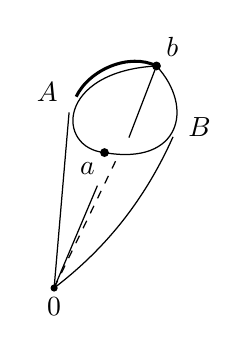
\begin{tikzpicture}[x=1cm,y=1cm,line width=.45pt]
\coordinate (o) at (0,0);
\coordinate (a) at (.64,1.72);
\coordinate (b) at (1.30,2.82);
\draw (a) .. controls (.02,1.78) and (.03,2.75) .. (b);
\draw[line width=1.1pt] (.28,2.43) .. controls (.45,2.78) and (.96,2.99) .. (b);
\draw (b) .. controls (1.79,2.29) and (1.60,1.55) .. (a);
\draw (o) -- (.19,2.23);
\draw (o) .. controls (.76,.58) and (1.21,1.25) .. (1.51,1.92);
\draw (b) -- (.95,1.91);
\draw[dashed] (o) -- (.78,1.61);
\draw (o) -- (.55,1.30);
\fill (a) circle (1.6pt);
\fill (b) circle (1.6pt);
\fill (o) circle (1.3pt);
\node[left] at (.17,2.49) {$A$};
\node[right] at (1.58,2.04) {$B$};
\node[below left] at (a) {$a$};
\node[above right] at (b) {$b$};
\node[below] at (o) {$0$};
\end{tikzpicture}}}

Pour tout $x\in X$, considérons \inserted{l'ens $I_x\subset I$} des $i\in I$ tels
que $X_i\ni x$ --- il y en a un nb fini, \deleted{et}
(par (1' a)), et l'ens de ces $\unsure{I|i}$ est filtrant
décroissant par (21 d), donc il y a
un plus petit $i\in I_x$ \deleted{tel que}, soit $i(x)$
\[
(25)\qquad i(x)=\text{plus petit des }i\in I\text{ tels que }x\in X_i.
\]
Soit d'autre part, pour tout $i\in I$
\mspage{53}
\scanpage{55}
\mspage{15}
\[
(26)\qquad
\underset{\text{fermé de }X_i}{\dot X_i\overset{\mathrm{def}}=\bigcup_{j<i}X_j},
\qquad
\underset{\text{ouvert de }X_i}{X_i^*\overset{\mathrm{def}}=X_i\setminus\dot X_i}.
\]

\margin{\uline{NB} On n'exclut pas que \unsure{certains} des $\unsure{X_i^*|X_i}$ soient $=\varnothing$ même si $X_i\ne\varnothing$. Sauf erreur, il n'y a pas d'\unsure{inconvénient} à remplacer $I$ par le sous-ens. \unsure{ord.} de $I$ \unsure{formé des} $i$ tels que $X_i^*\ne\varnothing$ \unsure{clairement} $(X_i)_{i\in I'}$ \deleted{\unsure{d'ailleurs}} \inserted{\unsure{satisfont}} \deleted{\unsure{satisfont}} aux $=$ conditions a) b) c) d).}

\uline{Proposition} Les $X_i^*$ sont mutuellement disjoints, et leur réunion est $X$. Si $x\in X$, $i(x)$ est aussi l'unique $i\in I$ tel que $x\in X_i^*$.

\uline{Dém.} Soit $x\in X_i^*\cap X_j^*$ ($i,j\in I$, $i\ne j$), donc \deleted{\unsure{alors}} $x\in X_i\cap X_j$ \deleted{(\unsure{car})}, donc $\exists k\leq i,j$ avec
\deleted{$\unsure{k\leq i\ \text{ou}\ k\leq j}$}
$x\in X_k$ si on avait $k=i$ on aurait $i\leq j$ donc $i<j$ absurde car $x\in X_j^*\subset X_j\setminus\unsure{X_i^*|X_i}$.
\unsure{Or|On a} $k<i$ donc $x\in X_i\setminus X_k$ ce qui contredit $x\in X_i^*$. Donc les $X_i^*$ mutuellement disjoints. D'ailleurs $x\in X_{i(x)}^*$ est trivial par définition de $i(x)$, d'où la prop.

On posera
\[
(27)\qquad
\left\{\begin{aligned}
\dot X_{\Delta_0}&=\coprod_{i\in I}\dot X_i\\
X_{\Delta_0}^*&=X_{\Delta_0}\setminus\dot X_{\Delta_0}=\coprod_{i\in I}X_i^*,
\end{aligned}\right.
\]
puis \deleted{\unsure{par}} plus généralement
\[
(28)\qquad
\left\{\begin{aligned}
\dot X_{\Delta_r}&=\text{image inverse de }\dot X_{\Delta_0}\text{ par}\\
&\qquad\unsure{\sigma_r|a_r}:X_{\Delta_r}\longrightarrow X_{\Delta_0}
\qquad\text{\uline{fermé} de }X_{\unsure{\Delta_r|\Delta_0}}\\
\underset{\text{ouvert de }X_{\Delta_r}}{X_{\Delta_r}^*}&=X_{\Delta_r}\setminus\dot X_{\Delta_r}=\text{image inv. de }X_{\unsure{X_0|\Delta_0}}^*\\
&\qquad\text{par }\unsure{\sigma_r|a_r}:X_{\Delta_r}\longrightarrow X_{\Delta_0}.
\end{aligned}\right.
\]
\mspage{54}
\scanpage{56}
Si
\[
\alpha:\Delta_{r'}\longrightarrow\Delta_r,\qquad \uuline{$\alpha(0)=0$},
\]
\[
(29)\qquad\left\{\begin{aligned}
&\text{alors}\qquad \alpha^*:X_{\Delta_r}\mathbin{\unsure{-|\longrightarrow}}X_{\Delta_{r'}}\qquad(\text{étale})\\
&\text{satisfait}\\
&\qquad\alpha^*(X_{\Delta_{r'}}^*)=X_{\Delta_r}^*,\quad\text{i.e. }\alpha^*(\dot X_{\Delta_{r'}})=\dot X_{\Delta_r}.
\end{aligned}\right.
\]

\deleted{\unsure{Dans le cas}}

\uline{NB} ``Moralement'', $X_{\Delta_r}^*$ représente une sorte de partie ``non singulière'' de $X_{\Delta_r}$, $\unsure{X_{\Delta_r}|\dot X_{\Delta_r}}$ la partie singulière ou ``bord''. On fera attention que les $X_{\Delta_r}^*$ ne \uline{forment} \uline{pas} un espace semi-simplicial.

Pourtant, notre propos est, dans une certaine mesure, de reconstituer $X$ à partir des ``strates ouvertes'' $X_i^*$ dans $X$, dans l'esprit du n° 1 (où il y a deux strates $X_0=Y$ et $X_1=X$, \deleted{$Y\subset X$ \unsure{fermé}} \inserted{($Y\subset X$ inclusion} fermée)), et on a donc $Y=Y^*$, $X^*=X\setminus Y$ comme dans les notations du loc. cit, où il y avait lieu d'introduire $V_{Y,X}$.
\mspage{55}
\scanpage{57}
\mspage{16}
3. \uline{Stratifications globales} : \uline{introduction aux tubes}

On garde les notations précédentes.

Pour tt couple $(i\leq j)\in I\times I$, considérons
\[
(1)\qquad \overline V_{i,j}=V_{X_i,X_j}\qquad
\begin{gathered}\text{voisinage tubulaire}\\\text{de }X_i\text{ dans }X_j\end{gathered}
\]
(cf § 1), et posons
\[
(2)\qquad\dot V_{i,j}=\deleted{\unsure{\overline V_{ij}}}\ \overline V_{ij}\cap\bigl(\deleted{\unsure{R_j}}\inserted{R_{i,j}^{\deleted{\unsure{*}}}}\bigr)=\overline V_{ij}\cap R_i
\]
où on pose, pour $i,j\in I$
\[
(3)\qquad R_{i,j}^{\deleted{\unsure{*}}}=\left(
\underbrace{\bigcup_{\substack{k\in I\ \text{tels que}\\\deleted{\unsure{X_k}}\ X_k\not\supset X_i}}X_k}_{\substack{R_i\ \text{partie fermée}\\\text{de }X}}
\right)\cap X_j
\]
\deleted{$(\unsure{\bigcup}_{k<j\ \unsure{\text{tel q}}}$}

\margin{\uline{NB} On a aussi
\[
(3\mathrm{bis})\qquad R_{ij}=\bigcup_{\substack{\uline{$k<j$}\\\text{tel que }X_k\cap X_i\ne X_i}}X_k\subset\dot X_j.
\]}

On notera qu'on a
\[
(4)\qquad R_{i\deleted{j}}\cap X_i=R_{ij}\cap X_i=\dot X_i.
\]
En effet, si $X_k\not\supset X_i$ i.e. $X_k\cap X_i\subsetneq X_i$, comme $X_k\cap X_i=\bigcup_{l\leq k,i}X_l$, on voit que \deleted{$X_k\cap X_i\ \unsure{\text{et}}\ l<i$} $l\leq k,i$ implique $X_l\subsetneq X_i$, d'où $l<i$ et $X_l\subset\dot X_i$, donc $X_k\cap X_i\subset\unsure{\dot X|\dot X_i}$, d'où $R_i\cap X_i\subset\dot X_i$ — l'inclusion en sens inverse étant triviale.
\mspage{56}
\scanpage{58}
On posera \deleted{enfin}
\[
(5)\qquad V_{ij}=\overline V_{ij}\setminus\dot V_{ij}=\overline V_{ij}-\overline V_{ij}\cap R_{ij}
\]
qui est donc un espace infinitésimal autour de
\[
(6)\qquad V_{ij}\cap X_i=X_i^*.
\]
Je poserai enfin
\[
(7)\qquad\begin{aligned}
V_{ij}^*&=\overline V_{ij}\setminus\bigcup_{\deleted{\unsure{i}}\,\uline{$k$}<j}X_k\cap\overline V_{ij}\\
&=\overset{\deleted{\unsure{-}}}{\overline V}_{ij}\setminus\dot X_j\\
&=V_{ij}\cap X_j^*\subset V_{i,j}.
\end{aligned}
\]
Notons que pour $i=j$, on trouve
\[
(8)\qquad\overline V_{ii}=X_i,\quad\dot V_{i,i}=\dot X_i,\quad\uline{$V_{i,i}=V_{i,i}^*=X_i^*$}
\]
Nos ``pierres'' de construction, dans une première étape, vont être les $V_{ij}^*$, $V_{ij}$ avec les inclusions évidentes
\diagram{(9)\qquad\begin{tikzcd}[column sep=large,row sep=small]
& X_i^*\arrow[d,"\text{``âme''}"]\\
\unsure{V_{ij}^*|X_{ij}^*}\arrow[r]\arrow[d] & V_{i,j}\\
X_j^* &
\end{tikzcd}}
,
ces pierres \unsure{comprenant|comprennent} \inserted{les} $X_i^*$ comme
\mspage{57}
\scanpage{59}
\mspage{17}
cas particuliers, en faisant $i=j$.

À vrai dire, je vois maintenant que ces fameuses pierres telles qu'elles sont des \unsure{côtes|cotes} mal taillées — ils sont trop \unsure{généraux|généreux}, \unsure{ou pas assez. Pas assez} pour contenir les morceaux $\unsure{V|\overline V}_{d_*,d''_*}^{d'_*}\unsure{\simeq|\cong}\widetilde N_{d_*;(d'_0,d''_0)}\mid D_{d_*}^*$ de ($\mathrm{Str}_\infty$ p. 84) — trop en ce sens, que l'on peut s'en tirer avec des ``pierres'' plus petites pour certaines des précédentes, correspondant au cas où $j$ est un \uline{successeur} de $i$ (i.e. $\nexists h$ avec $i<h<j$).
Ces pierres sont \inserted{\uline{particulièrement}} intéressantes, en ce sens que pour des hypothèses de lissité et de locale trivialité normale (ou ``équisingularité'') convenables du type standart (et sûrement réalisables p. ex. pour tt variété alg. complexe, munie de sous-variétés alg. complexes fermées)), $V_{i,j}^*$ \deleted{\unsure{est}} homéomorphe${}^*$ à un fibré sur $X_i^*$ (qui est une variété topologique) à fibre une variété topologique, et même à fibre un cylindre ouvert : $\mathbb R\times C_{ij}$ \inserted{($\simeq Z_{ij}^*=Z_{i,j}\setminus\{\unsure{z|0}\}$)} (où $C_{ij}$ est une \uline{variété top. compacte} (NB $V_{ij}$ serait homéomorphe à un fibré en \uline{cônes} sur $C_{ij}$ \ldots). Quand $j$ n'est pas un successeur de $i$, alors $C_{ij}$ sera encore une variété, mais non compacte. Quand

\margin{\uline{\uuline{NB}} Mais ce dessin (dans le domaine réel) dessine une situation pas tellement vraisemblable — qui ne correspond pas vraiment aux ``hyp. \ldots\ convenables du type standart'' la \unsure{str.te|str.} $X_i$
\figure{\begin{tikzpicture}[x=1cm,y=1cm]
\draw (0,0)--(3,0);\fill (1.5,0) circle (1.8pt);
\node[above] at (.25,0) {$X_i$};
\end{tikzpicture}}
devrait se décomposer en tous cas en deux.}

\margin{${}^*$ du moins si $X_i^*=X_i$, i.e. $\dot X_i=\varnothing$, sinon on peut avoir \deleted{\unsure{des cas}} des situations comme dans le dessin
\figure{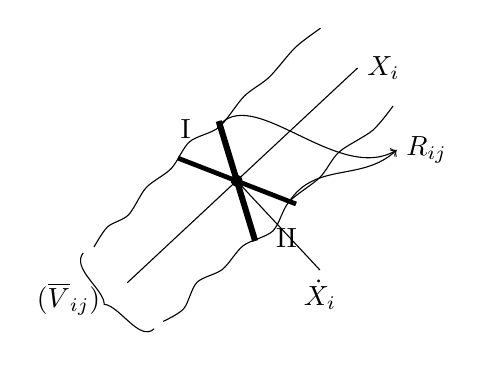
\begin{tikzpicture}[x=1cm,y=1cm,rotate=43]
\draw (0,0)--(4,0) node[right] {$X_i$};
\draw plot[smooth] coordinates {(0,.62)(.3,.69)(.6,.62)(1,.72)(1.4,.68)(1.8,.77)(2.2,.65)(2.7,.72)(3.1,.68)(3.6,.73)(4,.69)};
\draw plot[smooth] coordinates {(0,-.67)(.3,-.73)(.65,-.6)(1,-.7)(1.4,-.66)(1.8,-.78)(2.2,-.65)(2.7,-.69)(3.1,-.62)(3.6,-.71)(4,-.66)};
\draw[line width=1.7pt] (1.55,.72)--(2.25,-.73);
\draw[line width=2.2pt] (1.55,-.72)--(2.25,.71);
\fill (1.9,0) circle (2.1pt);
\node at (1.87,.92) {$\mathrm I$};\node at (1.87,-.96) {$\mathrm{II}$};
\draw[->] (1.9,-1.55)--(1.9,-.06);\node[below] at (1.9,-1.55) {$\dot X_i$};
\draw[->] (2.18,.66) .. controls (2.9,.8) and (2.8,-.91) .. (3.65,-1.1);
\draw[->] (2.2,-.65) .. controls (2.8,-.5) and (3.05,-1.1) .. (3.65,-1.1);
\node[right] at (3.65,-1.1) {$R_{ij}$};
\draw (-.15,-.66) .. controls (-.4,-.66) and (-.27,-.15) .. (-.4,0) .. controls (-.27,.14) and (-.4,.62) .. (-.15,.66);
\node[left] at (-.3,0) {$(\unsure{\overline V_{ij}})$};
\end{tikzpicture}}
où dans $V_{ij}^*$ il y a des morceaux suppl. ``idiots'' I et II \ldots}
\mspage{58}
\scanpage{60}
aux espaces (plutôt, germes d'espaces ou topos) \deleted{$\unsure{V_{ij}}$} plus généraux que les $V_{ij}^*$ (et les $V_{ij}$), ce sont les suivants : on considère
\[
i\leq j\leq k\qquad\text{d'où}\qquad X_i\subset X_j\subset X_k
\]
on prend
\[
(10)\qquad V_{i,k}^j\overset{\mathrm{def}}=\overline V_{X_i,X_k}\setminus(R_{\deleted{\unsure{j}}\inserted{i},k}\cup\unsure{S_{j,k}|\Sigma_{j,k}})\ \deleted{\unsure{m}}
\]
où $R_{i,k}$ est défini dans (3) (3bis), et où
\[
(11)\qquad S_{j,k}\overset{\mathrm{def}}=\bigcup_{\substack{l\in I\\\text{avec}\\j\leq l<k}}X_l
\]
\margin{(\uline{NB} $S_{j,k}=\varnothing$ si $j=k$\\
$S_{j,k}=X_j$ si $k$ succ. de $j$)}

On a, en comparant avec (3bis), une \deleted{\unsure{partition}} \inserted{\unsure{partition}} de l'ens. $I^{(k)}\overset{\mathrm{def}}=\{l\in I\mid\unsure{l<k|l\leq k}\}$ en deux parties,
\[
\unsure{I^{*(k)'}|I^{(k)'}}=\{l\in I^{(k)}\mid X_l\not\supset X_j\}\quad\text{et}\quad
\unsure{I^{(k)''}|I^{(k)'}}=\{l\in I^{(k)}\mid X_l\supset X_j\},
\]
et on a
\[
(12)\qquad\left\{\begin{aligned}
R_{j,k}&=\bigcup_{l\in I^{(k)'}}X_l\\
S_{j,k}&=\bigcup_{l\in I^{(k)''}}X_l,
\end{aligned}\right.
\qquad\begin{gathered}
\text{Donc }R_{j,k}\cup S_{j,k}=\dot X_k\\
(\text{aussi }R_{j,k}\cap S_{j,k}=\dot X_{\unsure{i|j}})
\end{gathered}
\]
\deleted{$\unsure{V_{ij}}$} On a donc
\[
(13)\qquad V_{i,k}^i=V_{i,k}^*,\qquad V_{i,k}^k=V_{i,k},
\]
\margin{d'où $V_{i,i}^i=V_{i,i}=V_{i,i}^*=X_i^*$.}

$V_{i,k}^j$ a encore tendance à être \deleted{\unsure{un}} homéomorphe (ou du moins, \unsure{homotope}, ou homéomorphe en un sens affaibli \unsure{de germes|de genre}, qu'il faudrait dégager\ldots) à un fibré loc. trivial de base $X_i^*$, mais comme c'est déjà dans le cas $V_{i,k}^k=V_{i,k}$) à fibre pouvant être \uline{singulière}. Dans le cas de $V_{i,k}^k$,
\mspage{59}
\scanpage{61}
\figure{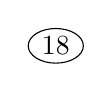
\begin{tikzpicture}\draw (0,0) ellipse (.35cm and .22cm);\node at (0,0) {\mspage{18}};\end{tikzpicture}}
avec $k$ successeur de $i$, il s'agit de singularité isolée, mais dans le cas de $V_{i,k}^k$ \unsure{général}, on peut trouver des singularités de type arbitraire bien sûr en fibre (prendre $X_i=X_i^*$ réduit à un pt !) — ce qui diminue l'intérêt, dans le cas de stratifications \unsure{tant soit peu} générales, des $V_{i,k}^j$ généraux comme ``pierres''. Les $V_{i,k}^{\unsure{j|i}}=V_{i,k}^*$ sont déjà plus intéressants, car \deleted{\unsure{ce sont}} c'est essentiellement un \inserted{germe d'} ouvert de $X_k^*$, donc non singulier — ce qui s'exprimera par le fait qu'on l'obtient comme un fibré sur $X_i^*$ non singulier, à fibre non singulière $V_{\unsure{z|Z},Z_{i,k}}^*$ \ldots

Donc nous allons dans la suite systématiquement essayer d'exprimer le maximum avec les $X_i^*$ et \inserted{les} $V_{ij}$, $V_{i,j}^*$ ``élémentaires'' ($j$ successeur de $i$), puis voir si certaines expressions peuvent prendre une forme plus sympathique en utilisant aussi \inserted{les $X_i^*$ et} les $V_{ij}$, $V_{i,j}^*$ avec $i\leq j$ sans plus — et dans un dernier temps seulement, peut-être (en égard au cas des diviseurs à croisements normaux) voir comment les $V_{i,k}^j$ s'insèrent dans ce formalisme.
\mspage{60}
\scanpage{62}
Posons déjà
\[
(14)\qquad\left\{\begin{aligned}
V_{\Delta_1}&=\coprod_{\substack{(i,j)\in I^2\\i\leq j}}V_{i,j}\\
\overset{\deleted{\unsure{V}}}{V}_{\Delta_1}^*&=\coprod_{\substack{(i,j)\in I^2\\i\leq j}}V_{i,j}^*\underset{\text{ouvert}}{\subset}V_{\Delta_1}
\end{aligned}\right.
\]
on a donc
\diagram{(15)\qquad\begin{tikzcd}[column sep=large,row sep=large]
V_{\Delta_1}^*\arrow[r,hook]\arrow[d] & V_{\Delta_1}\arrow[d,dashed] & X_{\Delta_0}^*\arrow[l]\arrow[dl,dashed]\\
\unsure{X_{\Delta_0}^*|V_{\Delta_0}^*}\arrow[r,dashed] & X &
\arrow[from=2-1,to=2-2,phantom,"("{pos=.12}]\arrow[from=2-2,to=2-3,phantom,")"{pos=.05}]
\end{tikzcd}}
\diagram{\deleted{\unsure{(16)}\qquad\begin{tikzcd}
V_{\Delta_1} & X_{\Delta_0}^*\arrow[l]
\end{tikzcd}}}
qui reflètent les diagrammes
\diagram{(17)\qquad\begin{tikzpicture}
\node[inner sep=5mm] (d) {\begin{tikzcd}[column sep=large,row sep=large]
V_{i,j}^*\arrow[r]\arrow[d] & V_{ij}\arrow[d,dashed] & X_i^*\arrow[l]\arrow[dl,dashed]\\
X_j^*\arrow[r,dashed] & X &
\arrow[from=2-1,to=2-2,phantom,"("{pos=.12}]\arrow[from=2-2,to=2-3,phantom,")"{pos=.05}]
\end{tikzcd}};
\draw (d.north west) rectangle (d.south east);
\draw[->] (d.north west)--(d.west);
\end{tikzpicture}}

\margin{\uline{NB} La forme
\diagram{\begin{tikzcd}[column sep=small,row sep=small]
&\bullet\arrow[d]\\
\bullet\arrow[r]\arrow[d]&\bullet\\
\bullet&
\end{tikzcd}}
est peut être plus suggestive.}

\deleted{\unsure{On a}} Finalement, on n'est pas sûr que les notations (14) \unsure{soient|sont} bien utiles — de \unsure{tte|toute} façon le carré de (15) n'a rien de cocartésien, car le diagramme en trait plein, qui est le diagramme ``somme''
\mspage{61}
\scanpage{63}
\figure{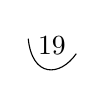
\begin{tikzpicture}\draw (-.30,.14) .. controls (-.25,-.35) and (.10,-.35) .. (.31,-.05);\node at (0,.05) {\mspage{19}};\end{tikzpicture}}
des diagrammes 17, donne une $\unsure{\underline{\mathrm{Lim}}|\underset{\longrightarrow}{\mathrm{Lim}}}$ qui se représente de $=$ comme espace somme, a peu de chances d'être homéo. à $X$ (p. ex. si $X$ conn\ldots) !

Les $\unsure{V_{j,k}^j|V_{i,k}^j}$ sont des germes de sous-espaces de $X$, leurs \unsure{seuls|seules} \deleted{\unsure{relations d'}} \inserted{morphismes} canoniques entre eux sont les morphismes d'inclusions — à quelle condition donc a-t-on
\[
(18)\qquad V_{i,k}^j\subset V_{i',k'}^{j'}
\]
pour
\[
(19)\qquad i\leq j\leq k,\qquad i'\leq j'\leq k'
\]
donnés ? Qu'en est-il pour les espaces élémentaires
\[
X_i^*,\quad V_{i,j}^*,\quad V_{i,j}\qquad(j\text{ successeur de }i)\ ?
\]
Je vais supposer pour simplifier les $X_i^*\ne\varnothing$.
\inserted{(\unsure{alors} $X_i\subset X_j\Longrightarrow i\leq j$ — car sinon on aurait $X_i^*=\varnothing$ justement\ldots)}
Il n'y a donc pas de relations d'inclusions entre les $X_i^*$ pour des indices distincts, \deleted{\unsure{si pour}} \inserted{Si} $V_{i,j}\subset V_{i',j'}$, passant aux ``pts'' \inserted{de $X$''} de ces germes d'espaces, il faut avoir $X_i^*\subset X_{i'}^*$ d'où $i=i'$, donc si on suppose que le germe d'un $X_j$ ($j$ successeur de $i$) le long de $X_i^*$ détermine déjà $j$ (ce qui est bien vraisemblable), on devra avoir aussi $j=j'$. De $=$, on voit que si $V_{ij}^*\subset V_{i',j'}^*$, leurs ens de pts d'adhérence, \deleted{\unsure{situés sur|à savoir} $\overline{X_i^*}$ et $\overline{X_{i'}^*}$}, compris entre $\overline{X_i^*}$ et $X_i$ \inserted{\unsure{resp.|pour} $\overline{X_{i'}^*}$ et $X_{i'}$}, sont en relation d'inclusion,
\mspage{62}
\scanpage{64}
dans le cas (vraisemblable) où $\overline{X_i^*}=X_i\ \forall i$, on aura donc $i\leq i'$, \deleted{\unsure{Dans le}} le cas $i=i'$, on voit comme tantôt qu'on aura (``vraisemblablement) $j=j'$. Mais le cas $i<\unsure{i'|j'}$ est-il possible ? Comme $V_{i,j}^*\subset X_j^*$ \inserted{$\varnothing\ne V_{i',j'}^*\subset X_{j'}^*$} on doit avoir $X_j^*\cap X_{j'}^*\ne\varnothing$ donc $j=j'$ (on aurait pu commencer par ça !)
\diagram{\begin{tikzcd}[column sep=small,row sep=small]
&&j'\\
&i'\arrow[ur,dash]&\\
i\arrow[ur,dash]\arrow[dr,dash]&&\\
&j&
\end{tikzcd}\qquad
\begin{tikzcd}[column sep=small,row sep=small]
&&X_{j'}\\
&X_{i'}\arrow[ur,dash]&\\
X_i\arrow[ur,dash]\arrow[dr,dash]&&\\
&X_j&
\end{tikzcd}}
donc \deleted{$\unsure{j}$} $i\leq i'<j=j'$ et par suite $i'=i$, puisque $j$ successeur de $i$.

On voit de $=$ que les seuls morphismes d'inclusion d'un $X_i^*$ dans un des deux autres types est
\diagram{\unsure{$\alpha)$}\qquad\begin{tikzcd}X_i^*\arrow[r]&V_{i,j}\end{tikzcd}
\deleted{(``vraisemblablement'')}
\inserted{(dans les ``cas vraisemblables'')}}
\deleted{Le seul} \inserted{il n'y a pas de} morphisme \inserted{d'un} $V_{ij}$ dans un des autres types, \deleted{est $V_{ij}$} enfin que le seul morphisme d'un $V_{ij}^*$ dans un des autres types est
\diagram{\unsure{$(\kappa\alpha)$|$(\beta_1)$}\qquad\begin{tikzcd}V_{ij}^*\arrow[r]&X_j^*\end{tikzcd}}
\diagram{\unsure{$(\mu\alpha)$|$(\beta_2)$}\qquad\begin{tikzcd}V_{ij}^*\arrow[r]&V_{ij}\end{tikzcd}}
en définitive, il n'y a pas lieu d'envisager d'autres morphismes entre ces \deleted{\unsure{p}} topos-pierres élémentaires.
\mspage{63}
\scanpage{65}
\figure{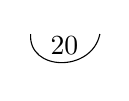
\begin{tikzpicture}\node at (0,0) {\mspage{20}};\draw (-.43,.15) .. controls (-.46,-.33) and (.35,-.34) .. (.45,.15);\end{tikzpicture}}

Ce sont aussi les \deleted{\unsure{diagr.}} flèches en traits pleins du diagramme fondamental (17)

Avec l'ens ordonné $I$, fabriquons donc un \deleted{ens ordonné} \uline{diagramme} dont les sommets sont \deleted{des ``lettres'' $\unsure{x|i}\ i^*$} des symboles \deleted{$\unsure{i_{**}|i_*}$} $[i]$, $[i,j]$, $[i,j]^*$, où $i,j\in I$, $j$ un succ. de $i$. Les flèches du diagramme sont des trois types qui sont toutes décrites ds
\[
(19)\qquad
\diagram{\begin{tikzcd}[column sep=large,row sep=large]
[i,j]^* \arrow[r] \arrow[d] & {[i,j]} & i^* \arrow[l] \\
{[j]^*} & &
\end{tikzcd}}
\]

Désignons par $\widetilde I$ ce diagramme, dont l'ens des sommets \deleted{s'identifie} a \deleted{$\unsure{I\times I_\Delta}$} \inserted{le card.} $\operatorname{card}I+2\nu$ \deleted{\unsure{card.}} \inserted{où $\nu=\operatorname{card}$} de l'ens des drapeaux $(i<j)$ ``élémentaires'' i.e. tels que $j$ est successeur de $i$ et le nb des flèches est $3\nu$. Si $I$ contient exactement deux élts $i,j$ avec $i<j$, \inserted{i.e. $I\simeq\Delta_1$,} ce diagramme \unsure{est en.|est env.} (19). Si $I=\Delta_r=(0,1,\ldots,r)$, on trouve (en employant maintenant les symboles pour les $X_i^*,V_{ij}^*,V_{ij}$ qui réalisent le diagramme)

\mspage{64}
\scanpage{66}
\diagram{\deleted{\begin{tikzcd}[column sep=small]
\unsure{V_{0,1}^*|V} \arrow[r] & V_{0,1} & X_0^* \arrow[l]
\end{tikzcd}}}

\margin{\uline{NB} ou mieux
\diagram{\begin{tikzcd}[row sep=small,column sep=small]
X_0^* \arrow[d] \arrow[r,dash] & {} \\
V_{01} & V_{01}^* \arrow[l] \arrow[d] \\
{} & X_1^* & {} \arrow[l]
\end{tikzcd}}}

\[
(20)\qquad
\diagram{\begin{tikzcd}[column sep=.3em,row sep=1.2em]
X_0^* \arrow[r] & \underset{\unsure{\updownarrow}}{V_{0,1}^*} & V_{0,1}^* \arrow[l] \arrow[d] & & & & & & & \\
& & X_1^* \arrow[r] & V_{1,2} & V_{1,2}^* \arrow[l] \arrow[d] & & & & & \\
& & & & X_2^* \arrow[r] & V_{2,3} & V_{2,3}^* \arrow[l] \arrow[d] & & & \\
& & & & & & X_3^* & & & \\
& & & \widetilde\Delta_n & & & \cdots & {} \arrow[d] & & \\
& & & & & & & X_{n-1}^* \arrow[r] & V_{n-1,n} & V_{n-1,n}^* \arrow[l] \arrow[d] \\
& & & & & & & & & X_n^*
\end{tikzcd}}
\]

Si $I$ est le diagramme
\diagram{\begin{tikzcd}[column sep=small,row sep=small]
& a \\
\unsure{0|\bullet} \arrow[ru] \arrow[rd] & \\
& b
\end{tikzcd}}, on trouve
\[
(21)\qquad
\diagram{\begin{tikzcd}[column sep=small,row sep=large]
\deleted{X_0^*} & V_{0,b}^* \arrow[r,phantom,"{\unsure{\to|-}}" description] \arrow[d] & V_{0,b} & X_0^* \arrow[l] \arrow[r] & V_{0,a} & V_{0,a}^* \arrow[l] \arrow[d] \\
& X_b^* & & & & X_a^*
\end{tikzcd}}
\]

Si $I$ est le diagramme
\diagram{\begin{tikzcd}[column sep=small,row sep=small]
a\mathord\cdot \arrow[rd] & \\
& c \\
b \arrow[ru,leftrightarrow] &
\end{tikzcd}}, on trouve
\[
(22)\qquad
\diagram{\begin{tikzcd}[column sep=large,row sep=large]
X_a^* \arrow[d] & & X_b^* \arrow[d] \\
V_{a,c} \arrow[d,leftrightarrow] & & V_{b,c} \\
V_{a,c}^* \arrow[r] & X_c^* & V_{b,c}^* \arrow[u] \arrow[l]
\end{tikzcd}},
\]
etc.

\deleted{La première chose qu'on aimerait \unsure{préciser|vérifier} est le} Supposons qu'on dispose sur $I$ d'une fonction à valeurs entières

\mspage{65}
\scanpage{67}
\mspage{21}
\[
(23)\qquad I\xrightarrow{d}\mathbb Z
\qquad (\text{i.e. } I=\coprod_m I_m)
\]
jouant le rôle d'une fonction dimension (on aurait une présentation en quelque sorte duale avec une fonction type codimension), satisfaisant la condition
\[
(24)\qquad\text{Si }i,j\in I\text{ et }i\leq j,\text{ alors }d(j)=d(i)+1\Longleftrightarrow j\text{ succ. de }i
\]
Posons alors, pour $m,n_{\deleted{\unsure{2|q}}}\in\mathbb Z$
\[
(25)\qquad\left\{\begin{aligned}
X_m^*&=\coprod_{\substack{i\in I_m\\\deleted{\unsure{d(i)}}}}X_i^*\\[1.5em]
V_{m,\deleted{\unsure{n}}\inserted{m+1}}^{\deleted{\unsure{*}}}&=\coprod_{\substack{(i,j)\in I\times I\\i\leq j,\ d(i)=m\\d(j)=m+1}}V_{i,j}\\[1.5em]
V_{m,m+1}^*&=\coprod_{\substack{i,j\text{ comme}\\\text{dessus}}}V_{ij}^*
\end{aligned}\right.
\]
de sorte qu'on a les diagrammes
\[
\underset{(\mathrm{Diag})_m}{(26)}\qquad
\diagram{\begin{tikzcd}[column sep=large,row sep=large]
X_m^* \arrow[r] & V_{m,m+1}^{\deleted{\unsure{*}}} & V_{m,m+1}^* \arrow[l] \arrow[d] \\
& & X_{m+1}^*
\end{tikzcd}}
\]
s'insérant dans un diagramme commun \inserted{qui n'est autre que (20),} infini en principe, mais que nous écrirons sous forme finie en \deleted{\unsure{présumant|privilégiant}} \unsure{simplifiant|simplifier} \deleted{$I$ fini}, \inserted{$d(I)$ \unsure{fini et} $\subset\mathbb N$)} et en n'écrivant pas les \deleted{\unsure{composantes}} \inserted{parties du diagramme} correspondant à des sommets occupés par des espaces vides :

\mspage{66}
\scanpage{68}
Dans le cas d'une fonction \uline{codimension} (\uline{$d(j)=j-1$} si $j$ succ. de $i$) on \deleted{peut} considère des $V_{\unsure{d|g},d-1},V_{d,d-1}^*$ au lieu des $V_{d,d+1},V_{d,\unsure{d+1}}^*$, et le diagramme prend la forme

\deleted{(27)} (Cas d'une fonction codimension)
\[
(27)\qquad
\diagram{\begin{tikzcd}[column sep=.5em,row sep=1.8em]
X_n^* \arrow[r] & V_{n,n-1} & V_{\unsure{n+n-1|n,n-1}}^* \arrow[l] \arrow[d] & & & & & \\
& & X_{n-1}^* \arrow[r] & V_{n-1,n-2} & V_{n-1,\unsure{n-2}}^* \arrow[l] \arrow[d] & & & \\
& & & & \unsure{X_{n-1}^*|X_{m-1}^*} & & & \\
& & & & \cdots & {} \arrow[d] & & \\
& & & & & X_1^* \arrow[r] & V_{1,0} & V_{1,0}^* \arrow[l] \arrow[d] \\
& & & & & & & X_0^*
\end{tikzcd}}
\]

\mspage{67}
\scanpage{69}
\mspage{22}
\uline{Th. de recollement des tubes} (\unsure{1\textsuperscript{ère}|1\textsuperscript{ière}} version) Considérons le diagramme de type $\widetilde I$, formé par les $X_i^*,V_{i,j}^*,V_{i,j}$ ($i,j\in I$, $j$ un successeur de $i$) et les trois types de flèches y figurant (en trait plein) ds (17). Alors $X$ s'identifie au \deleted{topos} \inserted{topos} $\underset{\longrightarrow}{\mathrm{Lim}}$ de ces topos.

\margin{Pour que cet énoncé \unsure{puisse prendre} un sens précis, il \unsure{faut} sans doute supp. $X$ \uline{sobre}, i.e. déterminé par $\operatorname{Top}(X)\ldots$}

\deleted{Faute de disposer de définitions en forme pour les voisinages tubulaires, je vais faire une démonstration, lorsqu'on \deleted{\unsure{pose} $X$} remplace \deleted{\unsure{les}} $V_{ij}$ par des \inserted{vrais} vrais ouverts de $X_j$ de la forme $\bar V_{i,j}\setminus R_{i,j}\cap\bar V_{i,j}$, où $\bar V_{i,j}$ est un voisinage de $X_i$ dans $X_j$, et qu'on pose $U_{ij}^*=U_{ij}\setminus X_i^*$. \deleted{Alors} \deleted{\unsure{des voisinages}}}

On va en donner une démonstration heuristique ci-dessous. Mais avant de le faire, je vais le généraliser, en un énoncé qui permet d'exprimer \unsure{également} les ``topos \unsure{canoniques|coconiques}'' associés à la \unsure{stratification}, en termes du système inductif de type $\widetilde I$ formé des topos élémentaires.

\mspage{68}
\scanpage{70}
\mspage{23}
\unsure{2|4}. \uline{Topos canoniques associés à une stratification globale.}

On va montrer comment, à une \unsure{situation} stratifiée donnée, on peut en associer d'autres.

A) Images inverses générales. Rappelons les axiomes utilisés jusqu'à présent :
\[
(1)\quad\left\{\begin{aligned}
&\text{a) }X_i\text{ fermés},\ (X_i)_{i\in I}\text{ loc. finie}\\
&\text{b) }i\leq j\Longrightarrow X_i\leq X_j\\
&\text{c) }X=\bigcup X_i\\
&\text{d) }\forall i,j\in I,\text{ on a }X_i\cap X_j=\bigcup_{\uline{\unsure{k|h}}<i,j}X_k
\end{aligned}\right.
\]

Notons que pour tt $X'$ au-dessus de $X$, la famille des
\[
(2)\qquad X'_i\overset{\mathrm{def}}=\deleted{\unsure{X\times X}}X_i\times_X X'
\]
satisfait les $\unsure{=^{\mathrm s}|\overline{\mathrm m}^{\mathrm s}}$ conditions.

D'ailleurs le système $\frac12$ \unsure{simple|simpl.} des $X_{\Delta_r}$ a comme image inverse celui des $X'_{\Delta_r}$, défini par les $X'_i$, \deleted{\unsure{d}} i.e. des iso
\[
(3)\quad\left\{\begin{aligned}
X'_{\Delta_r}&\simeq X_{\Delta_r}\times_X X'\\
X'^{*}_{\Delta_r}&\simeq X^*_{\Delta_r}\times_X X'\\
\dot X'_{\Delta_r}&=\dot X_{\Delta_r}\times_X X'
\end{aligned}\right.
\]

\mspage{69}
\scanpage{71}
\uline{NB} Nous appliquerons ces remarques surtout au cas où $X'$ est un ouvert de $X$. C'est pour pouvoir prendre de telles images inverses sans ennui, qu'il n'aurait pas été commode de supposer les $X_i$ ou les $X_i^*$ non vides, ou encore que $\unsure{I|i}\mapsto X_i$ est un \uline{plongt} d'ens ordonnés $I\hookrightarrow\unsure{\mathcal P|\mathfrak P}(X)$.

Lorsque $X'\to X$ est une imm. loc\textsuperscript{le} \deleted{\unsure{p}} \inserted{propre} \deleted{(\unsure{plus gén.}} \inserted{mais \uline{\uuline{pas}}} (\unsure{ou} une imm. ouverte !) alors la formation des images inverses des parties \deleted{\unsure{les}} fermées de $X$ commute à la formation des voisinages tubulaires d'une telle partie dans une autre. Notons d'ailleurs que pour $i<j$, on aura (sans hyp. d'ailleurs que $X'-X$ soit une imm. local)
\[
(4)\quad\left\{\begin{aligned}
R'_{ij}&=R_{ij}\times_X X'\\
S'_{ij}&=S_{ij}\times_X X'
\end{aligned}\right.,
\]
\margin{Il y a ici une propriété formelle importante des tubes qu'il faut vérifier --- \unsure{ça est valable} pour les topos définis \unsure{comme} germes d'espaces \unsure{en dehors hyp. métriques} (p.ex. $X$ compact --- \unsure{brrr!|barré!})}

d'où, dans le cas d'une imm. local, \inserted{propre,} des iso
\[
(5)\quad\left\{\begin{aligned}
V'^{\deleted{\unsure{*}}}_{i,j}&\simeq V_{i,j}\times_X X'\\
V'^{*}_{i,j}&\simeq V^*_{i,j}\times_X X'
\end{aligned}\right.\qquad i\leq j
\]

\mspage{70}
\scanpage{72}
\mspage{24}
et plus généralement
\[
(6)\quad V'{}^{j}_{i,k}\simeq V^{j}_{i,k}\times_X X',
\]
\unsure{tant qu'à faire}.

Ceci montre en particulier que la démonstration du th. de recollement, du th. énoncé p.22, est une question \uline{locale} sur $X$ \textcircled{$*$} --- ce qui permet p.ex. de nous réduire au cas où \deleted{\unsure{I}} \uline{$I$ est fini}.

\margin{\textcircled{$*$} \uuline{non}, ce n'est pas absolument clair, car les \unsure{restrictions} \unsure{au dessus} d'un ouvert ne \unsure{commutent} pas tt. à fait à la formation des topos ``limites''\dots C'est un \unsure{panneau|piège} \unsure{dans lequel} j'ai tendance à tomber, depuis le début de \unsure{mes} réflexions \unsure{sur les} \unsure{croisements normaux}\dots}

\deleted{Considérons p.ex. le cas où $X'=$}

B) \uline{Cas d'un} $X_{I'}$. \deleted{Soit}

Soit $I'$ une partie de $I$ telle que
\[
(7)\quad i\leq j\in I'\quad\Longrightarrow\quad i\in I'
\]
et soit
\[
(8)\quad X_{I'}=\bigcup_{i\in I'}X_i\qquad\text{(partie fermée de $X$)}
\]
On a bien sûr
\[
(9)\quad I'\subset I''\quad\Longrightarrow\quad X_{I'}\subset X_{I''},
\]
plus gén\textsuperscript{t}.
\[
(\unsure{10|9})\quad X_{I'\cup I''}=X_{I'}\cup X_{I''}
\]
plus gén.
\[
\left\{\begin{aligned}
\deleted{\unsure{\bigcup_\alpha}}X_{\bigcup_\alpha I'_\alpha}&=\bigcup_\alpha X_{I'_\alpha}\\
\text{aussi}\quad X_{\varnothing}&=\varnothing
\end{aligned}\right.
\]
et aussi
\[
(\unsure{9|11})\quad X_{I'\cap I''}=X_{I'}\cap X_{I''}\qquad
\left(\text{donc, }X_{\deleted{\unsure{\varnothing}}I}=X\right)
\]
grâce à (1 d). Dans ces formules,

\mspage{71}
\scanpage{73}
$I'$, $I''$, les $I'_\alpha$ sont des parties de $I$ satisfaisant (7) (des \uline{cribles} de $I$)

Si dans A) on prend $X'=X$, il est plus commode de travailler avec la stratification de $X'$ définie par les $X_i$ où $i\in I'$ --- Il est clair que les \unsure{conditions} (11) relatives à $X'=X_{I'}$ sont satisfaites. Les ``parties cribles'' de $X'$ pour cette stratification, ou pour celle induite au sens général des espaces au dessus de $X$, sont les $\unsure{=^{\mathrm s}|\overline{\mathrm m}^{\mathrm s}}$ --- ce sont \inserted{donc} les traces \deleted{\unsure{inverses}} \inserted{sur} $X'=X_{I'}$ des parties-cribles de l'espace stratifié $X$.

Ici, les espaces élémentaires pour la stratification de type $I'$ de \deleted{\unsure{X}} $X'=X_{\unsure{I'|J'}}$, sont les espaces
\[
(12)\quad \figure{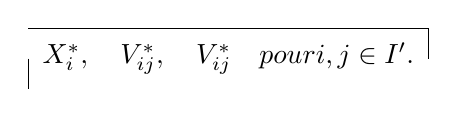
\begin{tikzpicture}
\node[inner sep=5pt] (f) {$X_i^*,\quad V_{ij}^*,\quad V_{ij}^{\deleted{\unsure{*}}}\quad\text{pour }i,j\in I'.$};
\draw (f.north west)--(f.north east)--(f.east);
\draw (f.west)--(f.south west);
\end{tikzpicture}}
\]

\deleted{Combinant les deux opérations, \unsure{on a} p.ex. une stratification pour \unsure{tt} ouvert $U'$ d'un $X'=X_{I'}$, avec les espaces élémentaires associés, qui sont donc les
\[
(13)\quad U'\cap X_i^*,\quad U'\cap V_{ij}^*,\quad U'\cap V_{ij}\qquad(i,j\in I')
\]}

\mspage{72}
\scanpage{74}
\mspage{25}
\unsure{Revenons|Revenant} pour un instant à $X$, et considérons \unsure{l'ens} \deleted{\unsure{de}} $I_0$ des $i\in I$ tel que $X_i=\varnothing$. C'est un crible, et on a $X_i^*=\varnothing$, $V_{ij}^*=V_{ij}=\varnothing$ si $i\in I_0$. Donc négligeant les espaces vides, on voit que le diagramme de type $\widetilde I$ défini par l'espace stratifié $X$ ne change pas \unsure{ess\textsuperscript{t}.} en remplaçant $I$ par $I\setminus I_0$, ou plus gén par $I\setminus I'_0$, où $I'_0\subset\unsure{I'|I_0}$ est un crible, ce qui donne lieu à un diagramme $\widetilde{I\setminus I'_0}$ qui est \uline{contenu} dans $\widetilde I$ (cela est vrai pour \uline{tt} crible de $I$).

Si p.ex. on a deux cribles
\[
(\unsure{14})\quad I''\subset I'\subset I
\]
d'où
\[
(\unsure{15})\quad X_{I''}\subset X_{I'}\quad\text{et}\quad U_{I',I''}\overset{\mathrm{def}}{=}X_{I'}\setminus X_{I''},
\]
on peut \deleted{\unsure{sur}} (et on va) sur $U_{I',I''}$ regarder plutôt la \deleted{filtration} \inserted{stratification} de type $I'\setminus I''$, définie par les
\deleted{\[
X_{i'}\setminus X_{i'}\cap X_{I''}\quad(i'\in I')\subset X
\]}
\[
(\unsure{16})\quad X_{i',\deleted{\unsure{X}}\inserted{I',\unsure{I''|U''}}}=X_{i'}\setminus X_{i'}\cap X_{I''}\subset U_{I',I''}
\]
dont les topos élémentaires sont donc les $X_{i'}^*$ $(i'\in I'\setminus I'')$ et des $V^*_{i',j',X'}$, $V_{i',j',X'}$

\mspage{73}
\scanpage{75}
associés aux couples $(i',j')$ avec $i'\in I'\setminus I''$, $j'$ successeur de $i'$, On a
\diagram{\(\displaystyle (17)\quad\left\{\vcenter{\hbox{\begin{tikzcd}[row sep=large,column sep=large]
V_{i',j',X'} \arrow[r,hook] \arrow[d,phantom,"\cup"] & V_{i',j'} \arrow[d,phantom,"\cup"]\\
V^*_{i',j',X'} \arrow[r,hook] & V^*_{i',j'}
\end{tikzcd}}}\right.\)}

\margin{$\Vert$}
mais il n'est pas clair en général que ce soient \deleted{des} $\unsure{\overline{\mathrm m}}$ \inserted{\uline{seulement}} des équivalences d'homotopie\dots Donc il faut mieux ne pas trop s'avancer quand il s'agit de comparer les constructibles sur un $X_{I'}$, et sur un $U_{I',I''}=X_{I'}\setminus X_{I''}$.

Je vais me dispenser par \unsure{la suite} de \deleted{\unsure{m'étendre}} \inserted{regarder} plus particulièrement ce qui se passe en \unsure{s'induisant} ainsi sur un ouvert $U_{I',I''}$\dots

C) \uline{Les} $V^{I'''}_{I',I''}$.

On suppose \unsure{donné|donnés} des cribles
\diagram{\begin{tikzcd}[column sep=small,row sep=small]
& I' \arrow[dr,phantom,"\subset"{description}] & &\\
(18) & & I'' \arrow[r,phantom,"\subset"{description}] & I,\\
& I''' \arrow[ur,phantom,"\subset"{description}] & &
\end{tikzcd}}
d'où
\diagram{\begin{tikzcd}[column sep=small,row sep=small]
& X_{I'} \arrow[dr,phantom,"\subset"{description}] & &\\
(19) & & X_{I''} \arrow[r,hook] & X_I=X\\
& X_{I'''} \arrow[ur,phantom,"\subset"{description}] & &
\end{tikzcd}}

\mspage{74}
